\section{Experiments}
\label{sec:experiments}

We evaluate the protocol's central claim: that encryption protects each client's contribution at no cost to
the shared model's accuracy, where one-shot differentially private federated learning must trade accuracy for
the same protection. The evaluation tests that claim and the design choices behind it. We ask, in order: what
fine-tuning the pretrained layers and selecting among depth-one candidate aggregates add over the naive
one-shot average; how the method behaves under heterogeneity, a poisoned client, and the trajectory budget;
what the cryptographic protocol costs in time and communication, including against encrypted
transfer-learning peers; how much the one remaining surface, the released model, leaks; and what the method
reaches at the published setups of prior one-shot methods and at billion-parameter scale. Throughout, the
question is not whether the global model attains the highest possible test
accuracy, but whether the clients jointly obtain a single model close to a centrally fine-tuned one, in one
round, with cryptographic privacy that adds no accuracy cost.

\subsection{Setup}
\label{sec:setup}

\paragraph{No public data.} Every client starts from the \emph{same} public pretrained backbone with a
zero-initialized low-rank adapter and a freshly initialized head, the standard adapter initialization
$\thz$, which carries no client data and classifies at chance. Each client fine-tunes the adapter and head
on its own private data for a bounded $\Ksteps$ steps and uploads the encrypted displacement; the server
forms the depth-one weighted sum of \cref{eq:aggregate}. No labelled public set is used anywhere;
\cref{sec:publicbase} discusses the easier case in which a deployment does have one.

\paragraph{Tasks and backbones.} We evaluate on four text classification tasks of increasing label-space
size: AG-News (4 classes), TREC (6), DBpedia (14), and Banking77 (77), with two frozen encoders,
RoBERTa-base and MPNet, and on CIFAR-100 with a ViT vision backbone. Data are partitioned across clients by
a Dirichlet distribution over labels with concentration $\alpha$ (the standard label-skew partition: a
smaller $\alpha$ leaves each client a few dominant classes and almost none of the rest). Unless stated
otherwise there are $\Nc=10$ clients, the adapter is rank $8$, the trajectory is $\Ksteps=200$ steps, and
every number is averaged over three seeds.

\paragraph{What we report.} We report the test accuracy of the HE-IFD global model; the shared start $\thz$
classifies at chance, since it carries no task head. Two reference points frame it: a frozen-feature head
(a linear probe trained under the same protocol) and, as the ceiling, the same model fine-tuned centrally
on the pooled private data, what one party would obtain holding all of it. The two quantities of interest are
the \emph{increment} of HE-IFD over the frozen-feature head and the \emph{gap} below the centralized ceiling;
the centralized accuracy itself we give in the relevant captions rather than repeat in every row.
\Cref{tab:setup} lists the axes.

\begin{table}[t]
\centering
\caption{Evaluation axes. Each varies one dimension around the default ($\Nc=10$, rank-$8$ adapter,
$\Ksteps=200$, three seeds); no public data is used anywhere.}
\label{tab:setup}
\footnotesize
\begin{tabular}{p{0.26\linewidth}p{0.29\linewidth}p{0.30\linewidth}}
\toprule
Axis & Setting & Question it probes \\
\midrule
Trainable unit & head-only vs.\ rank-$\{4,8,16\}$ adapter & value of fine-tuning pretrained layers \\
Heterogeneity $\alpha$ & $0.05$ (severe) to $1.0$ (mild) & robustness to label skew \\
Clients $\Nc$ & $10,\ 20,\ 50,\ 100$ & scalability in participants \\
Trajectory $\Ksteps$ & $100,\ 200,\ 400$ & the bounded-step budget \\
\bottomrule
\end{tabular}
\normalsize
\end{table}

\subsection{The Value of Fine-Tuning the Pretrained Layers}
\label{sec:superior}

The design rests on two choices working together: adapting the backbone's own layers with a small
frozen-projection adapter (small enough to encrypt inexpensively, yet fine-tuning the pretrained
representation itself), and selecting among depth-one candidate aggregates after decryption rather than
committing to a fixed rule the blind server cannot adapt. \Cref{fig:increment} and \cref{tab:headline}
measure both at $\Nc=10$ and moderate heterogeneity, against the naive sample-weighted average and the
centralized ceiling.

\begin{figure}[t]
\centering
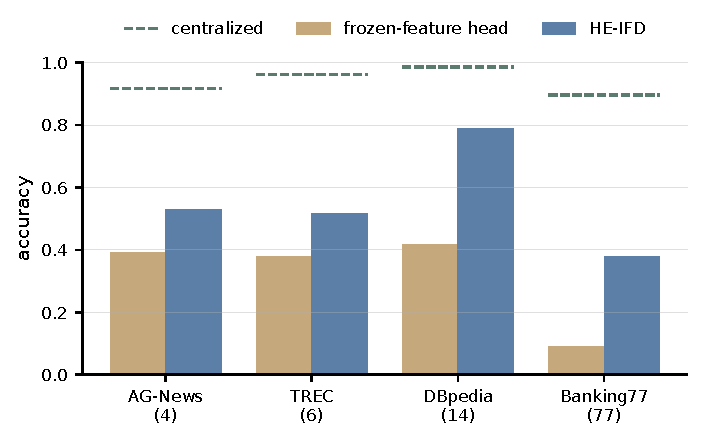
\includegraphics[width=\linewidth]{figures/fig_increment.pdf}
\caption{HE-IFD raises the single encrypted aggregation well above the chance start and above the naive
sample-weighted average; the gap to centralized grows with the size of the label space, and no client data
is shared.}
\label{fig:increment}
\end{figure}

\begin{table}[t]
\centering
\caption{HE-IFD against the naive one-shot aggregation and the centralized ceiling ($\Nc=10$, $\alpha=0.1$,
rank-$8$ frozen-projection adapter, three seeds). ``Naive'' is the plain sample-weighted average
($\lambda{=}1$, no candidate selection); HE-IFD is the client-selected candidate; $\pm$ is the seed standard
deviation; the gap is HE-IFD to centralized. Text tasks use frozen RoBERTa, CIFAR-100 a frozen ViT-B/16.}
\label{tab:headline}
\footnotesize
\begin{tabular}{lcccc}
\toprule
Task ($\Cc$) & naive avg & HE-IFD & centralized & gap \\
\midrule
AG-News (4)     & 0.51 & $\mathbf{0.75}{\pm}0.09$ & 0.91 & 0.16 \\
TREC (6)        & 0.51 & $\mathbf{0.72}{\pm}0.05$ & 0.95 & 0.23 \\
DBpedia (14)    & 0.80 & $\mathbf{0.93}{\pm}0.01$ & 0.99 & 0.06 \\
Banking77 (77)  & 0.39 & $\mathbf{0.77}{\pm}0.02$ & 0.88 & 0.11 \\
CIFAR-100 (100) & 0.47 & $\mathbf{0.78}{\pm}0.01$ & 0.87 & 0.09 \\
\bottomrule
\end{tabular}
\normalsize
\end{table}

Two effects combine in \cref{tab:headline}. First, fine-tuning the frozen backbone's own layers with a
small adapter raises the model far above the chance start: from a $\thz$ that classifies at chance to between
$0.72$ and $0.93$ across the four text tasks and $0.78$ on CIFAR-100, with only the small adapter and head
entering the encrypted combination, so the protocol and its cost do not change across tasks. Second, the
candidate set with client-side selection (\cref{sec:candidates}) raises the released model above the
naive sample-weighted average, by $0.24$ on AG-News, $0.21$ on TREC, $0.13$ on DBpedia and $0.38$ on
Banking77; the naive average is the combination that heterogeneity makes unstable, and the vote
selects the candidate that is robust to it. The remaining gap to the centralized fine-tune is small at moderate
label spaces ($0.06$ on the 14-class DBpedia) and is largest where a single round must cover many classes
each client barely observes; even there, freezing the adapter's projection and selecting a coverage-weighted
candidate hold the 77-class Banking77 gap to $0.11$, down from over $0.5$ for the naive average. HE-IFD
produces the model in one round, with no client exposing its data and with encryption that perturbs nothing.

\subsection{Heterogeneity and Client Count}
\label{sec:heterogeneity}

How much the released model trails the centralized one is governed by label skew, the axis the single
linear aggregation is most exposed to. \Cref{tab:het} sweeps the Dirichlet concentration on DBpedia at
$\Nc=10$. The accuracy degrades gracefully and monotonically, from $0.98$ when the data are near-uniform
($\alpha=1.0$, within $0.01$ of centralized) to $0.87$ under severe skew ($\alpha=0.05$), while the
centralized fine-tune barely moves. The gap the one-shot aggregation pays is therefore a property of
heterogeneity, small when each client sees most of the label space and widening only when each sees a sliver
of it; this is the same coverage effect that \cref{sec:basin} characterises, and the candidate selection
contains it rather than letting it collapse the model.

\begin{table}[t]
\centering
\caption{HE-IFD accuracy across label heterogeneity ($\Nc=10$) and client count ($\alpha=0.1$) on DBpedia,
three seeds; centralized $\approx 0.99$ throughout.}
\label{tab:het}
\footnotesize
\setlength{\tabcolsep}{5pt}
\begin{tabular}{lcccc@{\hskip 1.2em}lccc}
\toprule
\multicolumn{5}{c}{Heterogeneity $\alpha$} & \multicolumn{4}{c}{Clients $\Nc$} \\
\cmidrule(r){1-5}\cmidrule(l){6-9}
& 0.05 & 0.10 & 0.30 & 1.00 & & 10 & 20 & 50 \\
\midrule
HE-IFD & 0.87 & 0.93 & 0.96 & 0.98 & HE-IFD & 0.93 & 0.90 & 0.93 \\
\bottomrule
\end{tabular}
\normalsize
\end{table}

The aggregation is also stable as participants are added. Holding $\alpha=0.1$ and scaling the client count
from $10$ to $50$ (\cref{tab:het}, right), HE-IFD stays at $0.90$--$0.93$ with no downward trend, even as each
client's shard thins fivefold; the single linear combination neither destabilises nor washes out as $\Nc$
grows, and the protocol's cost (\cref{sec:fhe-cost}) is the only quantity that scales with it.

\subsection{Robustness to a Poisoned Client}
\label{sec:robust}

The same multi-candidate mechanism that selects the best aggregation rule also gives a measured defense
against a misbehaving client, at no homomorphic cost. We add to the candidate set the $\Nc$ leave-one-out
aggregates (\cref{sec:candidates}) and let one client (the one holding the largest shard, the worst case for
sample weighting) upload a crafted displacement instead of an honest one: a sign-flipped update, a
large-norm Gaussian, or one trained on label-flipped data. The honest clients vote on their local
holdouts over the plain aggregate and the $\Nc$ leave-one-out aggregates; the candidate that excludes
the attacker is selected whenever its exclusion improves the held-out accuracy.

\Cref{tab:poison} reports the result on DBpedia and AG-News at $\Nc=10$, three seeds. The undefended plain
aggregate is pulled down to $0.25$--$0.50$ depending on the attack, while the vote-selected model recovers
to within rounding of the attacker-free oracle, and the vote identifies and excludes the attacker in
$17$ of $18$ cells. The one miss is a Gaussian attack whose corruption was mild enough that including the
attacker still scored best on the holdouts, i.e. the vote kept it precisely because it was not harmful. This
is not a general Byzantine guarantee (it assumes an honest holdout majority and a single attacker), but it
shows the candidate machinery already absorbs a poisoning client that the blind server cannot filter.

\begin{table}[t]
\centering
\caption{Robustness to one poisoned client (DBpedia and AG-News, $\Nc=10$, $\alpha=0.1$, three seeds).
``Plain'' is the undefended sample-weighted aggregate that includes the attacker; ``HE-IFD'' is the
vote-selected leave-one-out candidate; ``oracle'' is the attacker-free aggregate; ``excluded'' counts how
often the vote dropped the attacker.}
\label{tab:poison}
\footnotesize
\begin{tabular}{lccccc}
\toprule
Attack & plain & HE-IFD & oracle & excluded \\
\midrule
sign-flip   & 0.25 & $\mathbf{0.65}$ & 0.65 & 6/6 \\
large-Gauss & 0.50 & $\mathbf{0.67}$ & 0.65 & 5/6 \\
label-flip  & 0.48 & $\mathbf{0.65}$ & 0.65 & 6/6 \\
\bottomrule
\end{tabular}
\normalsize
\end{table}

\subsection{Trajectory Length}
\label{sec:trajectory}

The trajectory length sets how far each client moves from the shared start before its displacement is
aggregated. \Cref{tab:traj} varies the step budget $\Ksteps$ on DBpedia: within the swept range a longer
trajectory helps monotonically, lifting HE-IFD from $0.91$ at $\Ksteps=100$ to $0.94$ at $\Ksteps=400$ and
narrowing the gap to centralized to $0.05$, the frozen backbone keeping even the longest trajectory's
displacements coherent enough to sum.

\begin{table}[t]
\centering
\caption{Trajectory length: HE-IFD accuracy (DBpedia, $\Nc=10$, $\alpha=0.1$);
centralized $\approx 0.99$.}
\label{tab:traj}
\footnotesize
\begin{tabular}{lcc}
\toprule
$\Ksteps$ & HE-IFD & gap \\
\midrule
100 & 0.91 & 0.08 \\
200 & 0.93 & 0.06 \\
400 & 0.94 & 0.05 \\
\bottomrule
\end{tabular}
\normalsize
\end{table}

\subsection{When Public Data Is Available}
\label{sec:publicbase}

We study the harder setting in which no public data exists, because that is where a one-shot encrypted
aggregation is actually needed. When a deployment does have a public labelled set, the problem is strictly
easier and standard recipes apply directly: the shared initialization can be warm-started on it, or a model
can be trained on the public data and then refined. With enough of it, training a model from scratch on
the public set is itself an option. We therefore treat public data as outside the method and rely on none of
it anywhere in this paper.

\subsection{Homomorphic-Encryption Implementation and Cost}
\label{sec:fhe-cost}

We do not simulate the cryptography. We implement the entire protocol end to end in real multiparty CKKS on
the Lattigo library~\cite{lattigo,mouchet2021multiparty}: distributed key generation, encryption under the
joint public key, the homomorphic weighted aggregation of \cref{eq:aggregate}, and threshold decryption by a
collective key-switch, and the decrypted aggregate matches the plaintext computation to within CKKS encoding
precision (verified below). The server's only cryptographic operation is that depth-one weighted sum, and its
cost is set entirely by the number of \emph{fine-tuned} parameters that enter a ciphertext, not by the frozen
backbone behind them. We measure the per-operation rates directly and calculate every reported configuration
from them, so a small adapter and head are inexpensive to encrypt whatever model they sit on.

\paragraph{Parameters and setup.} All figures use ring degree $2^{14}$ ($8192$ slots per ciphertext), a
modulus chain $\log Q=\{55,45\}$ with key-switch prime $\log P=\{61\}$, and scale $2^{45}$. The circuit is
multiplicative \emph{depth one} (one plaintext-scalar multiplication and a rescale, with no relinearization
and no bootstrapping), and decryption is $\Nc$-out-of-$\Nc$ (no single party can decrypt). Communication
figures are exact; timings are single-run wall-clock on one core of a commodity laptop CPU (Apple M4) and are
reported as indicative. The circuit uses no ciphertext rotations and no relinearization, and because the only
server operation is the one-shot aggregation, there is no encrypted training loop and hence no convergence
behaviour to report under encryption. The server accumulates the weighted sum as a streaming reduction,
holding at most two adapter-sized ciphertext sets at once (about $38$\,MiB), so its memory does not grow with
$\Nc$.

\paragraph{Communication.} A round is one upload and one download, and the protocol completes in a single
round. The per-client traffic is fixed by the trainable-parameter count: a unit of up to $8192$ parameters
is a single $0.5$\,MiB ciphertext. The headline configuration, a freeze-$A$ rank-$8$ adapter with a
classifier head (about $1.5\times10^5$ trainable parameters), occupies $19$ ciphertexts, or $9.5$\,MiB per
client; freezing the down-projection is what halves this relative to training both factors. Total traffic
scales linearly in the number of clients (\cref{tab:cost-comm}). The contrast with encrypted full-model
schemes is structural: on the same backbone, encrypting the full RoBERTa-base ($1.25\times10^8$ parameters)
would move about $7.5$\,GiB per client \emph{per round}, and such schemes run for many rounds, where HE-IFD
encrypts only the adapter and runs once (\cref{fig:comm}). The object stays small even on a billion-parameter
backbone: a freeze-$A$ adapter on the $0.5$B Qwen2.5 model is $26$ ciphertexts ($13$\,MiB), because only the
adapter is encrypted, never the backbone.

\begin{table}[t]
\centering
\caption{Per-client communication per round (multiparty CKKS, ring $2^{14}$, $0.5$\,MiB per ciphertext).
A round is one upload and one download; totals scale linearly in $\Nc$ (\cref{fig:comm}).}
\label{tab:cost-comm}
\footnotesize
\setlength{\tabcolsep}{3pt}
\begin{tabular}{lcc}
\toprule
Trainable unit & ciphertexts & up$=$down per client \\
\midrule
\textbf{freeze-$A$ adapter$+$head (RoBERTa)} & \textbf{19} & \textbf{$9.5$ MiB} \\
freeze-$A$ adapter$+$head (Qwen2.5-0.5B) & 26 & $13$ MiB \\
text head (4-class)   & 1  & $0.50$ MiB \\
vision head (100-class) & 10 & $5.0$ MiB \\
\bottomrule
\end{tabular}
\normalsize
\end{table}

\paragraph{Computation.} The server's homomorphic work is tens of milliseconds at deployment scale and stays
sub-second even at $\Nc=100$ (\cref{tab:cost-time}). The measured operations follow simple
laws: a client encrypts in about $2.1$\,ms per ciphertext (in parallel across clients), while the server
aggregation and the threshold decryption scale linearly in $\Nc\times(\text{ciphertexts/client})$, and the
one-time distributed key generation grows linearly in $\Nc$ at about $1$\,ms per party. From these rates the
freeze-$A$ adapter ($19$ ciphertexts) costs about $40$\,ms to encrypt per client and, at $\Nc=100$, about
$0.72$\,s to aggregate and $0.43$\,s to decrypt (\cref{tab:cost-time}). Emitting $k$ candidate aggregates
(\cref{sec:candidates}) costs $k$ threshold decryptions, so a dozen candidates add about half a second; there
is no bootstrapping anywhere in the protocol.

\begin{table}[t]
\centering
\caption{Computation time (ms, one CPU core, Apple M4). DKG is a one-time setup; the encrypt figure is per
client (clients encrypt in parallel); aggregation and decryption scale linearly in $\Nc\times$ciphertexts.}
\label{tab:cost-time}
\footnotesize
\setlength{\tabcolsep}{4pt}
\begin{tabular}{llcccc}
\toprule
Trainable unit & $\Nc$ & DKG & encrypt/client & aggregate & decrypt \\
\midrule
\textbf{freeze-$A$ adapter} & 10  & $11$ & $40$ & $76$  & $44$ \\
\textbf{freeze-$A$ adapter} & 100 & $96$ & $40$ & $717$ & $430$ \\
text head    & 10  & $13$ & $2.3$  & $3.9$   & $2.4$ \\
text head    & 100 & $96$ & $2.2$  & $38.9$  & $23.2$ \\
vision head  & 10  & $11$ & $21.5$ & $39.0$  & $24.6$ \\
vision head  & 100 & $98$ & $21.7$ & $382.2$ & $216.5$ \\
\bottomrule
\end{tabular}
\normalsize
\end{table}

\paragraph{Comparison with other encrypted schemes.} \Cref{tab:hecomm} places HE-IFD against the encrypted
federated-learning approaches. Two properties separate it from all of them. First, it is one-shot: it
encrypts a single contribution and runs one round, where encrypted-training schemes such as
POSEIDON~\cite{sav2021poseidon} run multiparty CKKS for many rounds, hours of wall-clock even on small
models, and aggregation schemes such as BatchCrypt, FedML-HE, and
FedSHE~\cite{zhang2020batchcrypt,jin2023fedml,wei2025fedshe} encrypt and sum updates on every round of an
iterative protocol. Second, it encrypts only the small adapter and head, not the full model: the per-client
object is $9.5$\,MiB against the gigabytes a full-model scheme moves on the same backbone, and there is no
bootstrapping because the circuit is depth one. The closest recent scheme, SHE-LoRA~\cite{li2025shelora},
also encrypts only adapter parameters, but it is multi-round and pays its encryption cost on every round, and
because it trains both adapter factors it carries the bilinear aggregation noise under encryption that our
frozen-projection design removes. The secure-aggregation primitive of~\cite{kemmaka2025hybagg}
is one-round but protects a per-round sum within an iterative protocol rather than a one-shot contribution.
\Cref{fig:comm} shows the per-round communication gap on a shared backbone, before the round-count multiplier
that further separates a one-round protocol from a multi-round one.

\begin{figure}[t]
\centering
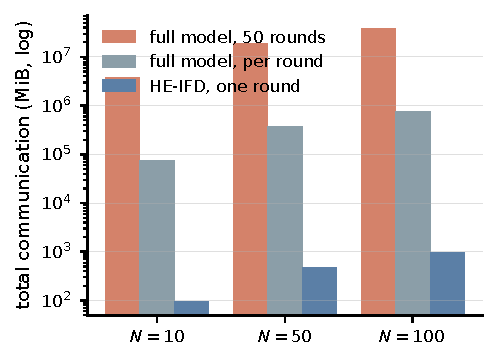
\includegraphics[width=\linewidth]{figures/fig_comm.pdf}
\caption{Total communication on a shared backbone (RoBERTa-base), calculated for CKKS ring $2^{14}$
($0.5$\,MiB per ciphertext; $50$ rounds for the iterative schemes). HE-IFD encrypts only the adapter and runs
once; full-model encrypted schemes move gigabytes per round (BatchCrypt, FedML-HE, FedSHE) to terabytes over
training (POSEIDON-style encrypted training).}
\label{fig:comm}
\end{figure}

\begin{table*}[t]
\centering
\caption{HE-IFD against encrypted federated-learning schemes. Communication is per client; HE-IFD's is
calculated for a freeze-$A$ adapter (RoBERTa-base, $19$ ciphertexts), the full-model figure for encrypting
the same backbone.}
\label{tab:hecomm}
\footnotesize
\begin{tabular}{lcccc}
\toprule
Method & crypto & encrypted object & rounds & comm/client \\
\midrule
\textbf{HE-IFD (ours)} & multiparty CKKS & adapter$+$head & \textbf{1} & \textbf{$9.5$ MiB} \\
SHE-LoRA~\cite{li2025shelora} & CKKS (selective) & adapter subset & many & per round \\
POSEIDON & multiparty CKKS & full model & many & GiB ($\sim$1.4 h) \\
BatchCrypt / FedML-HE / FedSHE & CKKS & full model & many & GiB / round \\
Hyb-Agg & multi-key CKKS & update sum & per round & secure sum \\
\bottomrule
\end{tabular}
\normalsize
\end{table*}

The encrypted object stays depth one and the server cost grows only with the ciphertext count, never with the
size of the frozen backbone the adapter sits in.

\paragraph{Comparison with encrypted transfer learning.} The closest cost comparison outside federated
learning is HETAL~\cite{lee2023hetal}, which solves the same structural problem --- fine-tuning a small
unit on frozen pretrained features without revealing the data behind it --- but places the encryption
around the \emph{optimizer}: the client encrypts its extracted features, and the server trains a softmax
head on the ciphertexts with an encrypted gradient method, approximated softmax, and bootstrapping.
\Cref{tab:hetal} sets the two designs and their reported costs side by side. HETAL reports $567$--$3442$\,s
of encrypted training across its five benchmarks on an NVIDIA A40 GPU with a 64-thread server CPU, with an
accuracy drop of up to $0.51\%$ against plaintext training on the same features. Our encrypted pipeline
(encrypt, aggregate, threshold-decrypt) takes about $0.16$\,s at $\Nc{=}10$ and $1.2$\,s at $\Nc{=}100$ on
one laptop CPU core, and is exact to a relative $\ell_2\approx10^{-9}$, because training happens in
plaintext on each client and only the finished displacement is ever encrypted. The comparison is indicative
rather than controlled: HETAL serves a single data owner outsourcing its training, whereas HE-IFD
aggregates across $\Nc$ mutually distrustful parties under a collective key, a setting HETAL does not
address, and HETAL trains only a classifier head where we also fine-tune adapters inside the backbone. But
it quantifies the structural point of \cref{sec:related-crypto}: moving the encryption boundary from the
optimizer to a one-shot aggregation removes the encrypted nonlinearities, the bootstrapping, and the GPU,
and replaces roughly hour-scale encrypted training with second-scale encrypted aggregation, three orders of
magnitude on weaker hardware. On the one benchmark the setups share, CIFAR-10 over a frozen ViT-Base
backbone, HETAL's encrypted head training reaches $96.57\%$ with all data at one party, and HE-IFD reaches
$96\%$ with the data split across five clients (\cref{tab:matched}).

\begin{table}[t]
\centering
\caption{Encrypted transfer learning against one-shot encrypted aggregation. HETAL figures are its paper's
own (HEaaN, ring $2^{16}$, NVIDIA A40 GPU $+$ 64-thread CPU); HE-IFD figures are from
\cref{tab:cost-time,tab:cost-comm} (Lattigo, ring $2^{14}$, one CPU core). The settings differ --- one data
owner outsourcing training vs.\ $\Nc$ mutually distrustful parties --- so the table contrasts where each
design pays its encryption cost.}
\label{tab:hetal}
\footnotesize
\setlength{\tabcolsep}{4pt}
\begin{tabular}{lcc}
\toprule
 & HETAL~\cite{lee2023hetal} & HE-IFD (ours) \\
\midrule
parties & $1$ owner $+$ server & $\Nc$ clients $+$ server \\
key & single-key CKKS & multiparty CKKS \\
encrypted object & features $+$ head & adapter displacement \\
trained under HE & softmax head & nothing \\
nonlinearity under HE & approx.\ softmax & none \\
bootstrapping & yes & no (depth one) \\
encrypted wall-clock & $567$--$3442$\,s & $0.16$--$1.2$\,s \\
accuracy vs.\ plaintext & $\le 0.51\%$ drop & exact ($\ell_2\!\approx\!10^{-9}$) \\
CIFAR-10, frozen ViT & $96.57\%$ (pooled) & $96\%$ (split, $\Nc{=}5$) \\
\bottomrule
\end{tabular}
\normalsize
\end{table}

\paragraph{Correctness.} The decrypted aggregate matches the plaintext computation to a relative $\ell_2$
error between $2.7\times10^{-9}$ ($\Nc=10$) and $2.6\times10^{-8}$ ($\Nc=100$). This is the encoding precision
of CKKS at scale $2^{45}$; it grows mildly with $\Nc$ as ciphertext additions and the key-switch smudging
noise accumulate, and it stays several orders of magnitude below any tolerance the decoded model is sensitive
to. Because the circuit is depth one, the error is not amplified.

\paragraph{Comparison with prior cryptographic federated learning.} The contrast with prior homomorphic
federated learning is structural, not incremental. Encrypted-training methods such as
POSEIDON~\cite{sav2021poseidon} reach comparable accuracy but through many rounds of homomorphic computation
that the source paper reports at roughly $1.4$ hours of wall-clock; secure-aggregation
primitives~\cite{kemmaka2025hybagg} sum updates once per round inside an iterative protocol. Our protocol runs
in a single round whose server computation is milliseconds and whose communication is a few megabytes,
because the only encrypted object is a bounded fine-tuning displacement of a small adapter, combined at
multiplicative depth one. The broader method-level positioning is in \cref{sec:related-positioning}.

\subsection{Residual Leakage: Measuring the Inference-Time Surface}
\label{sec:mia}

The design goal set in \cref{sec:intro} was to eliminate the training-time attack surface, and the protocol
achieves it by construction: no gradient, update, or data-derived summary is ever observable in plaintext,
and there is only one round in which anything is exchanged at all. What the cryptographic guarantee of
\cref{sec:security} does not cover is the final model, which every party obtains in the clear after
decryption. This is the \emph{inference-time} surface of \cref{sec:related-leakage}, and it is not a gap a
stronger mechanism could close: any protocol that hands separate parties a shared, useful model must move
knowledge between them, and a model that classifies categories a client never saw locally necessarily
encodes information about the data that taught it those categories. The meaningful question is not whether
this residual leakage is zero, which it cannot be, but how large it is, and the evidence of
\cref{sec:related-leakage} is that it is the weakest surface an adversary can be left with. This section
measures it directly.

Read as attack surfaces, the alternatives differ by orders of magnitude. Multi-round federated learning
publishes a fresh update every round, so a curious server or peer accumulates a long sequence of
training-time views of each client~\cite{shokri2017membership,nasr2019comprehensive}. One-shot methods that
rely on differential privacy ship, in a single object, essentially the whole of a client's local knowledge:
a synthetic copy of its data, or a noised model. HE-IFD exposes only the final aggregate: the per-client
displacements are encrypted and never appear in the clear, and because there is no alignment phase there is
no prototype channel either.

We measure the residual on that one open channel with membership-inference
attacks~\cite{yeom2018privacy,salem2019ml,carlini2022membership}, training the target and a population of
shadow models through the full federated pipeline and attacking the released model both with a loss-threshold
test and with the likelihood-ratio attack LiRA, under an external adversary and under the
\emph{fellow-client} adversary that brings its own data as a prior, the strongest the threat model of
\cref{sec:threat} admits (\cref{tab:mia}). On three of the four tasks the leakage is at the level of random
guessing: LiRA reaches an AUC of $0.49$--$0.50$ and a true-positive rate of about $1\%$ at a $1\%$
false-positive rate, indistinguishable from chance. On the 77-class Banking77 it is mildly elevated, to an
AUC of $0.59$ and a $3.4\%$ true-positive rate, the one task where coverage forces the model to memorise the
most per class, and exactly the task where the accuracy gap to centralized is largest; even there the signal
is small, and the fellow-client prior yields no measurable advantage over the external adversary. A
participant therefore learns little about another's membership from the shared model beyond what any usable
classifier of that data would reveal.

\begin{table}[t]
\centering
\caption{Membership inference against the released model (LiRA, $16$ shadow models, three seeds). AUC and
the true-positive rate at a $1\%$ false-positive rate, for an external adversary and a fellow client using
its own data as a prior. $0.50$ AUC and $1\%$ TPR are chance.}
\label{tab:mia}
\footnotesize
\begin{tabular}{lcccc}
\toprule
& \multicolumn{2}{c}{external} & \multicolumn{2}{c}{fellow client} \\
\cmidrule(r){2-3}\cmidrule(l){4-5}
Task ($\Cc$) & AUC & TPR@1\% & AUC & TPR@1\% \\
\midrule
AG-News (4)    & 0.50 & 0.9\% & 0.50 & 0.9\% \\
TREC (6)       & 0.49 & 0.7\% & 0.49 & 0.7\% \\
DBpedia (14)   & 0.50 & 0.9\% & 0.50 & 0.9\% \\
Banking77 (77) & 0.59 & 3.4\% & 0.59 & 3.4\% \\
\bottomrule
\end{tabular}
\normalsize
\end{table}

We do not claim the released model leaks nothing. A model that gives every client coverage of classes it
never observed must carry information about the data that supplied that coverage, and an adversary with
strong priors about a client's distribution can recover some of it; this is a property of useful shared
models, not of our protocol in particular. What the protocol guarantees is that this residual is the
\emph{entire} surface (not multiplied across the rounds of an iterative protocol, and not handed over
wholesale as released data), and driving the exposed surface down to that inherent floor, rather than
promising to remove a leak that cannot be removed when parties set out to build a common model, is the
privacy goal the design meets.

\subsection{Matched Setups and Scale}
\label{sec:matched}

The positioning of \cref{sec:related-positioning} separates the methods qualitatively; the accuracies each
paper reports are obtained at its own setup and do not compare directly. To make the comparison controlled,
we run HE-IFD at the \emph{published partitions}
of three one-shot methods, varying the dataset, client count, and Dirichlet $\alpha$ to match theirs while
keeping our model class (a frozen ViT-B/16 with a freeze-$A$ adapter, which we state). \Cref{tab:matched}
reports the result. At the data-free DENSE setup (CIFAR-10, $\Nc=5$) HE-IFD reaches $0.96$ against their
reported $0.50$/$0.60$; at the differentially private FedAUXfdp setup (CIFAR-10, $\Nc=20$, severe skew)
$0.94$ against $0.75$ at $\varepsilon{=}0.5$; and at the FedSD2C setup (Tiny-ImageNet, $\Nc=10$) $0.73$. The
gains owe much to the stronger frozen backbone, which is the point: the protocol's cryptographic and
communication structure carries unchanged onto a backbone that makes the task easy, where prior data-free and
differentially private one-shot methods cannot reach the same accuracy and, in the DP case, pay an explicit
budget for a weaker guarantee than encryption gives.

\begin{table}[t]
\centering
\caption{HE-IFD at the published partitions of prior one-shot methods (frozen ViT-B/16 $+$ freeze-$A$
adapter, three seeds). Comparator numbers are paper-verbatim at the cited setup.}
\label{tab:matched}
\footnotesize
\begin{tabular}{llcc}
\toprule
Matched setup & data, $\Nc$, $\alpha$ & HE-IFD & reported \\
\midrule
DENSE~\cite{zhang2022dense}     & CIFAR-10, 5, 0.1   & \textbf{0.96} & 0.50 \\
DENSE~\cite{zhang2022dense}     & CIFAR-10, 5, 0.3   & \textbf{0.96} & 0.60 \\
FedAUXfdp~\cite{hoech2022fedauxfdp} & CIFAR-10, 20, 0.04 & \textbf{0.94} & 0.75$^\ddagger$ \\
FedAUXfdp~\cite{hoech2022fedauxfdp} & CIFAR-10, 20, 0.16 & \textbf{0.96} & 0.75$^\ddagger$ \\
FedSD2C~\cite{zhang2024fedsd2c} & Tiny-ImageNet, 10, 0.1 & \textbf{0.73} & --- \\
FedSD2C~\cite{zhang2024fedsd2c} & Tiny-ImageNet, 10, 0.3 & \textbf{0.73} & --- \\
\bottomrule
\end{tabular}
\normalsize

\smallskip
\noindent\footnotesize $^\ddagger$FedAUXfdp at $\varepsilon{=}0.5$ on its CIFAR-10 setup.\normalsize
\end{table}

The protocol also carries to a billion-parameter-class backbone. On a frozen Qwen2.5-0.5B causal language
model with a freeze-$A$ adapter, HE-IFD reaches $0.87$--$0.88$ on DBpedia, where the naive average collapses
to $0.44$, and $0.71$--$0.72$ on AG-News, while the encrypted object stays at $26$ ciphertexts ($13$\,MiB):
the cost is set by the adapter, not by the $0.5$B backbone behind it, which is never encrypted.

\iffromscratch
\subsection{Beyond Pretrained Backbones}
\label{sec:fromscratch}

The protocol does not require a pretrained backbone; it requires a shared frame. Where clients instead train
a small network from a common random initialization, the same one-shot encrypted aggregation applies, but the
shared frame must be established rather than inherited. Without a pretrained representation the clients'
bounded updates are expressed in a coordinate system fixed only by the random seed, so agreeing on a useful
starting point reintroduces the kind of alignment step a pretrained backbone removes. We therefore present
pretrained fine-tuning as the primary setting and treat the from-scratch variant as a generalization whose
alignment cost is left to future work.
\fi

\subsection{Scope and Limitations}
\label{sec:scope}

Two boundaries follow from well-understood properties rather than incidental shortcomings. First, the single
linear aggregation pays a gap to centralized fine-tuning that widens with the size of the label space under
severe skew, because a client contributes signal only for classes it holds and the shared head is untrained;
this is an inherent property of combining bounded one-shot updates without an alignment phase, largest on the
77-class Banking77, and the coverage-weighted candidate contains it (to a gap of $0.11$) rather than removing
it. Second, the method fine-tunes a
pretrained backbone, so it inherits that backbone's fit to the task and applies to the label-groundable
foundation models used for transfer today rather than to a backbone with no relevant pretraining. Both are
stated where they apply; neither touches the privacy claim, which holds regardless of the accuracy the shared
model reaches.

\paragraph{Malicious and colluding clients.} Our cryptographic guarantees assume honest-but-curious
participants. An actively malicious client could upload a crafted displacement to bias the shared model, and
because the contributions are encrypted the server cannot inspect them, so plaintext outlier filtering does
not apply. The leave-one-out candidates of \cref{sec:robust} give a lightweight client-side defense that
already neutralises a single poisoning client without any server-side filtering, but it assumes an
honest-majority holdout and does not cover colluding or adaptive adversaries. Stronger guarantees compatible
with the encryption are left to future work: an upload-time norm bound enforced by a zero-knowledge proof,
which caps any single client's influence without revealing its update, and encrypted-domain robust
aggregation evaluated homomorphically. The one-shot structure shrinks the attack surface to a single round
but removes the cross-round consistency checks a multi-round protocol could use, and reconciling robust
aggregation with depth-one encryption is the open problem this direction must solve.
